\chapter{CALIDAD Y SEGURIDAD} 
\section{CALIDAD DE SOFTWARE}
\section{NORMAS DE CALIDAD}
\subsection{Usabilidad}

La usabilidad se evaluará a través de la escala de Likert, la cual permitirá medir la cantidad de clics necesarios para realizar distintas tareas en el software. De esta manera, se podrá valorar el nivel de satisfacción de los usuarios respecto al número de clics requeridos para completar dichas tareas. Además, esta escala proporcionará una visión clara sobre la eficiencia del diseño del software, ayudando a identificar áreas que podrían necesitar ajustes para mejorar la experiencia del usuario. La escala se define de la siguiente manera:

\begin{itemize}[label=$-$, left=0cm, labelsep = 0.9cm, topsep = 0pt, parsep = 0pt]
	\item \textbf{Muy insatisfecho:} Cinco o más clics, ya que las tareas requieren demasiados clics y son consideradas tediosas.		
	\item \textbf{Insatisfecho:} Cuatro clics, lo que indica que la tarea requiere más clics de los deseados y resulta algo incómoda.
	\item \textbf{Neutral:} Tres clics, una cantidad aceptable, aunque con margen de mejora.
	\item \textbf{Satisfecho:} Dos clics, considerado un número razonable que permite realizar la tarea de manera eficiente.
	\item \textbf{Muy satisfecho:} Un clic, ideal por ser altamente eficiente y requerir el mínimo esfuerzo.
\end{itemize}

\begin{longtable}{>{\centering\arraybackslash}m{5cm} >{\centering\arraybackslash}m{3cm} >{\centering\arraybackslash}m{3cm}}
	\caption[Número de Clics - Escala Likert]{\newline Número de Clics - Escala Likert} \label{tab:tabla_clics}\\
	\toprule
	\textbf{Tarea} & \textbf{Clics} & \textbf{Puntos}\\
	\midrule
	\endfirsthead
	
	\toprule
	\textbf{Tarea} & \textbf{Clics} & \textbf{Puntos}\\
	\midrule
	\endhead
	
	%\midrule
	%\multicolumn{3}{r}{\textit{Continúa en la siguiente página}} \\
	%\midrule
	%\endfoot
	
	\bottomrule
	\endlastfoot
	
	% Aquí se colocan las filas de la tabla, por ejemplo:
	Ingresar usuario      & 2 & 2 \\
	Registrar usuario     & 3 & 3 \\
	Registrar cliente     & 4 & 4 \\
	Venta de pasaje       & 3 & 3 \\
	Cancelar pasaje       & 2 & 2 \\
	Registrar encomienda  & 4 & 4 \\
	Generar reporte		  & 2 & 2 \\
	Cerrar sesión		  & 1 & 1 \\ \hline
	Total				  & 21 &  \\ \hline
	Promedio 			  &   & 2.62 \\
	
\end{longtable}
\vspace{-12pt}  % O el valor que necesites para ajustar
% Nota personalizada fuera de `\caption*{}`
% \textbf{Nota}: Esta es la nota de la tabla, explicando datos relevantes.

Se tiene un total de 21 clics para las tareas realizadas, con esto número obtenemos el promedio de clics de 2.62 y con este resultado concluimos que la usabilidad del sistema es "Satisfactorio".

\subsection{Portabilidad}

El proyecto es compatible con navegadores modernos asegurando una experiencia uniforme mediante el uso de estándares web, esto permite que el sistema funcione de manera consistente en distintos entornos, facilitando su acceso desde cualquier dispositivo. Además, se han implementado medidas para optimizar el rendimiento y minimizar inconsistencias entre navegadores, garantizando una experiencia fluida y eficiente para todos los usuarios, como podemos ver en las figuras \ref{fig:figura_brave}, \ref{fig:figura_edge} y \ref{fig:figura_celular}.

\vspace{3cm} % Agregar 1 cm de espacio entre el párrafo y la figura

\begin{figure}[!h] % 'H' del paquete 'float' para mantener posición	
	\caption[Navegador Brave]
	{\newline Navegador Brave.} % Leyenda en la parte superior
	\centering
	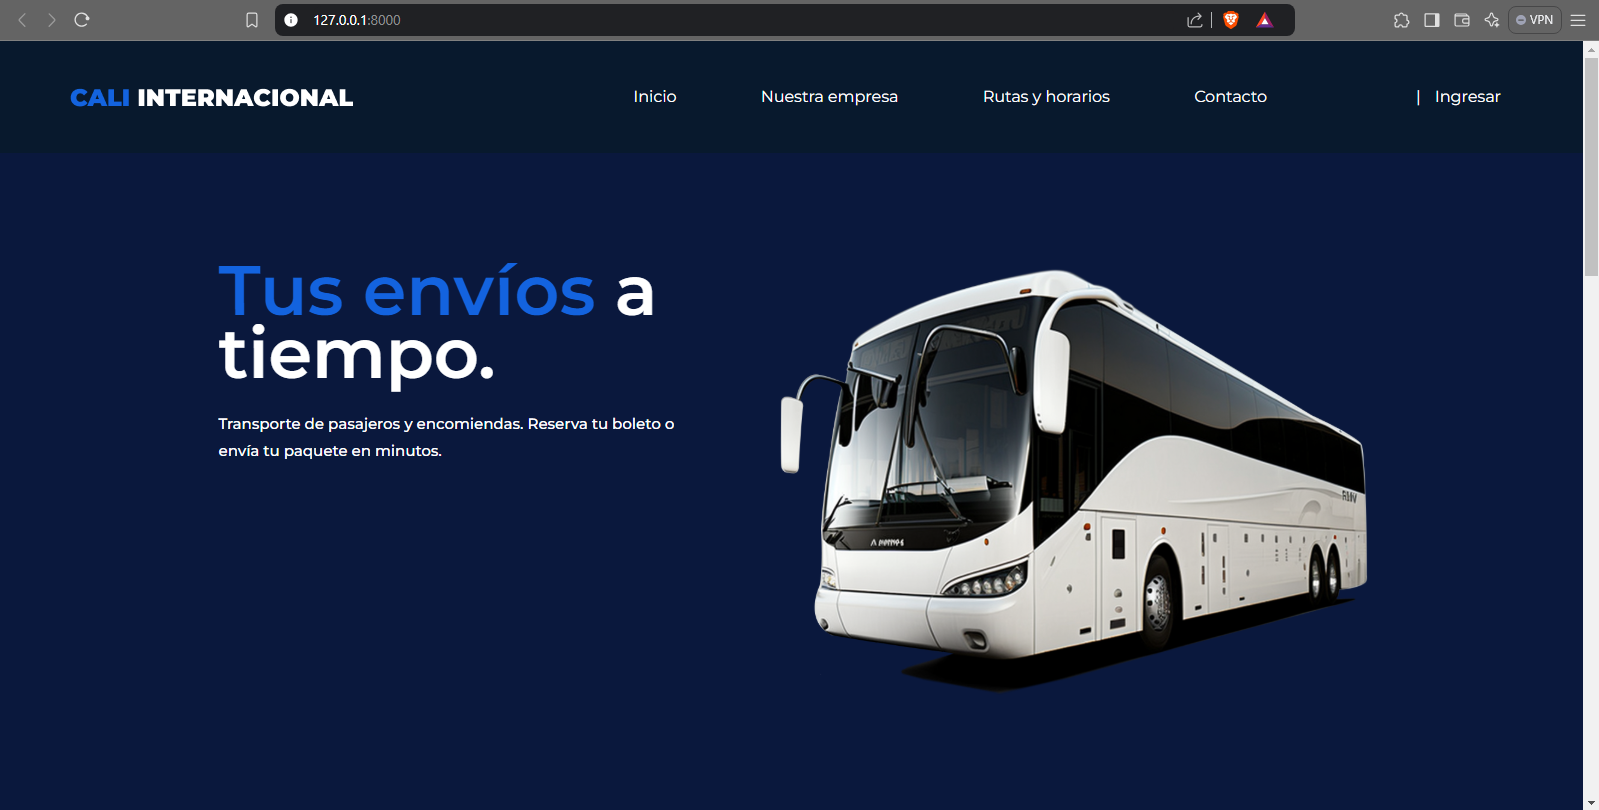
\includegraphics[width=0.95\textwidth]{imagenes/cap_3/brave.png} % Inserta una imagen
	
	%\begin{flushleft}
	%	\hspace{1.20cm} \textit{Nota.} al pie asociada con esta figura, explicando detalles adicionales. % Nota al pie para esta figura
	%\end{flushleft}
	% \vspace{-16pt}
	\label{fig:figura_brave} % Etiqueta para referencia cruzada
\end{figure}

\vspace{1cm} % Agregar 1 cm de espacio entre el párrafo y la figura

\begin{figure}[!h] % 'H' del paquete 'float' para mantener posición	
	\caption[Navegador Microsoft Edge]
	{\newline Navegador Microsoft Edge.} % Leyenda en la parte superior
	\centering
	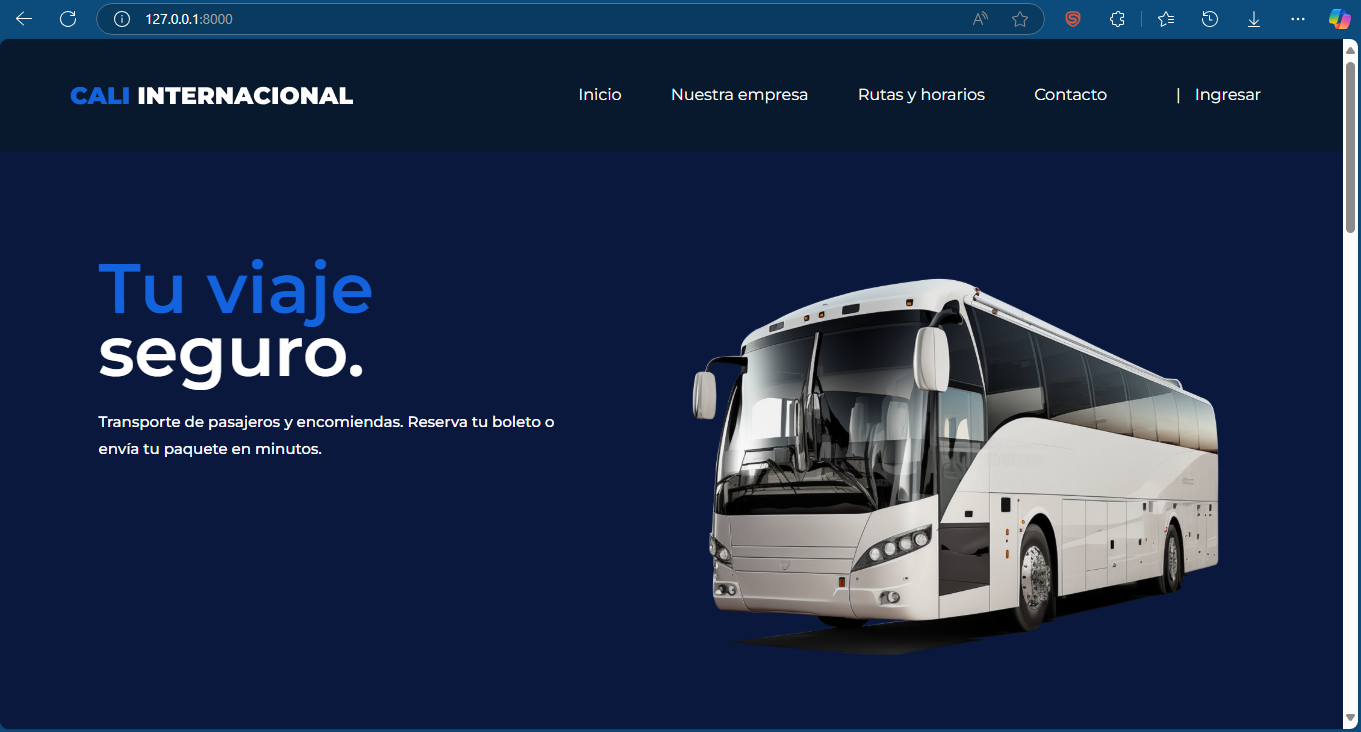
\includegraphics[width=0.95\textwidth]{imagenes/cap_3/edge.png} % Inserta una imagen
	
	%\begin{flushleft}
	%	\hspace{1.20cm} \textit{Nota.} al pie asociada con esta figura, explicando detalles adicionales. % Nota al pie para esta figura
	%\end{flushleft}
	\vspace{16pt}
	\label{fig:figura_edge} % Etiqueta para referencia cruzada
\end{figure}

\vspace{6cm} % Agregar 1 cm de espacio entre el párrafo y la figura

\begin{figure}[!h] % 'H' del paquete 'float' para mantener posición	
	\caption[Navegador Chrome - Móvil]
	{\newline Navegador Chrome - Móvil.} % Leyenda en la parte superior
	\centering
	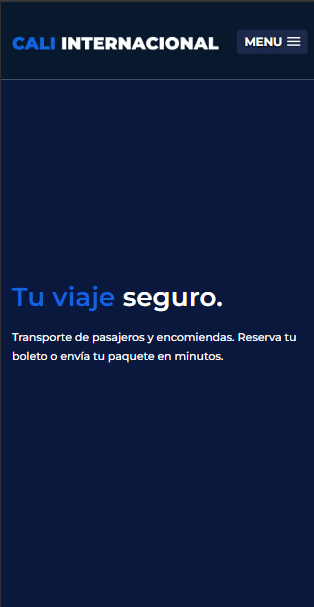
\includegraphics[width=0.4\textwidth]{imagenes/cap_3/celular.png} % Inserta una imagen
	
	%\begin{flushleft}
	%	\hspace{1.20cm} \textit{Nota.} al pie asociada con esta figura, explicando detalles adicionales. % Nota al pie para esta figura
	%\end{flushleft}
	\vspace{-16pt}
	\label{fig:figura_celular} % Etiqueta para referencia cruzada
\end{figure}

\vspace{0.3cm} % Agregar 1 cm de espacio entre el párrafo y la figura


\section{SEGURIDAD}

Implementar un sistema en línea accesible para los clientes, que permita realizar la compra de pasajes y la gestión de reservas desde cualquier dispositivo conectado a Internet. Esto no solo facilitará el acceso a los servicios de la empresa, sino que también incrementará su competitividad en el mercado al adaptarse a las expectativas modernas de los usuarios.

Realizar backups semestrales de la base de datos, garantizando que toda la información del sistema esté protegida frente a posibles pérdidas o fallos. Estos respaldos deben almacenarse en ubicaciones seguras, preferentemente en servidores externos o en la nube, para asegurar la recuperación efectiva de datos en caso de emergencias.

Desarrollar un sistema de chat en línea que brinde soporte en tiempo real a los usuarios, permitiéndoles resolver dudas, reportar problemas o recibir asistencia durante el proceso de compra y reserva. Este canal de comunicación directa mejorará la experiencia del cliente y reforzará la percepción de calidad del servicio ofrecido por la empresa.

Evaluar la posibilidad de automatizar las notificaciones a los clientes a través de correos electrónicos o mensajes de texto, informándoles sobre el estado de sus reservas o encomiendas, así como cualquier actualización en los servicios de la empresa. Esto contribuirá a mantener una comunicación efectiva con los usuarios.

\begin{figure}[!h] % 'H' del paquete 'float' para mantener posición	
	\caption[Interfaz gráfica - Cambio de contraseña]
	{\newline Interfaz gráfica - Cambio de contraseña.} % Leyenda en la parte superior
	\centering
	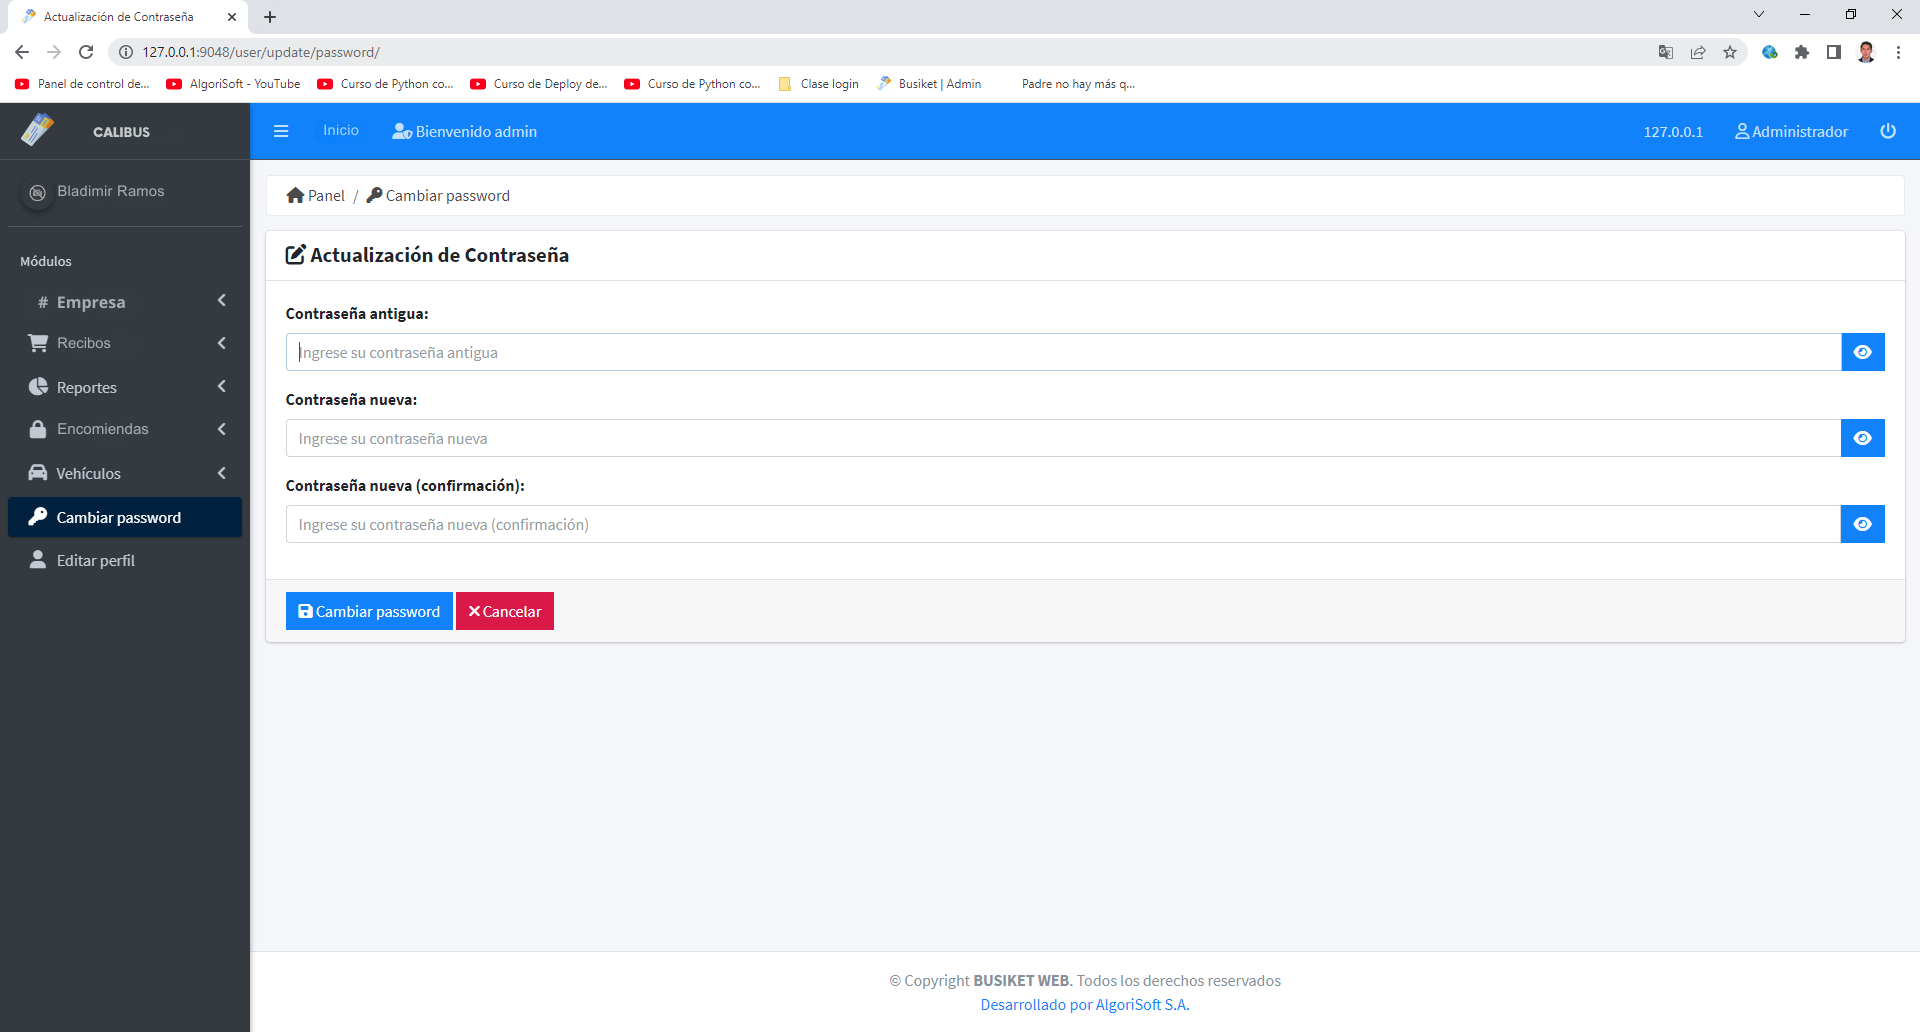
\includegraphics[width=0.85\textwidth]{imagenes/cap_3/Img_calibus/CALIBUS09.png} % Inserta una imagen
	
	\begin{flushleft}
		%\hspace{1.20cm} \textbf{Nota.} Organigrama obtenido en entrevista con el administrador. % Nota al pie para esta figura
	\end{flushleft}
	\vspace{-16pt}
	\label{fig:cali40} % Etiqueta para referencia cruzada
\end{figure}

\vspace{-0.6cm} % Agregar 1 cm de espacio entre el párrafo y la figura


 \begin{figure}[!h] % 'H' del paquete 'float' para mantener posición	
	\caption[Interfaz gráfica - Lista de accesos]
	{\newline Interfaz gráfica - Lista de accesos.} % Leyenda en la parte superior
	\centering
	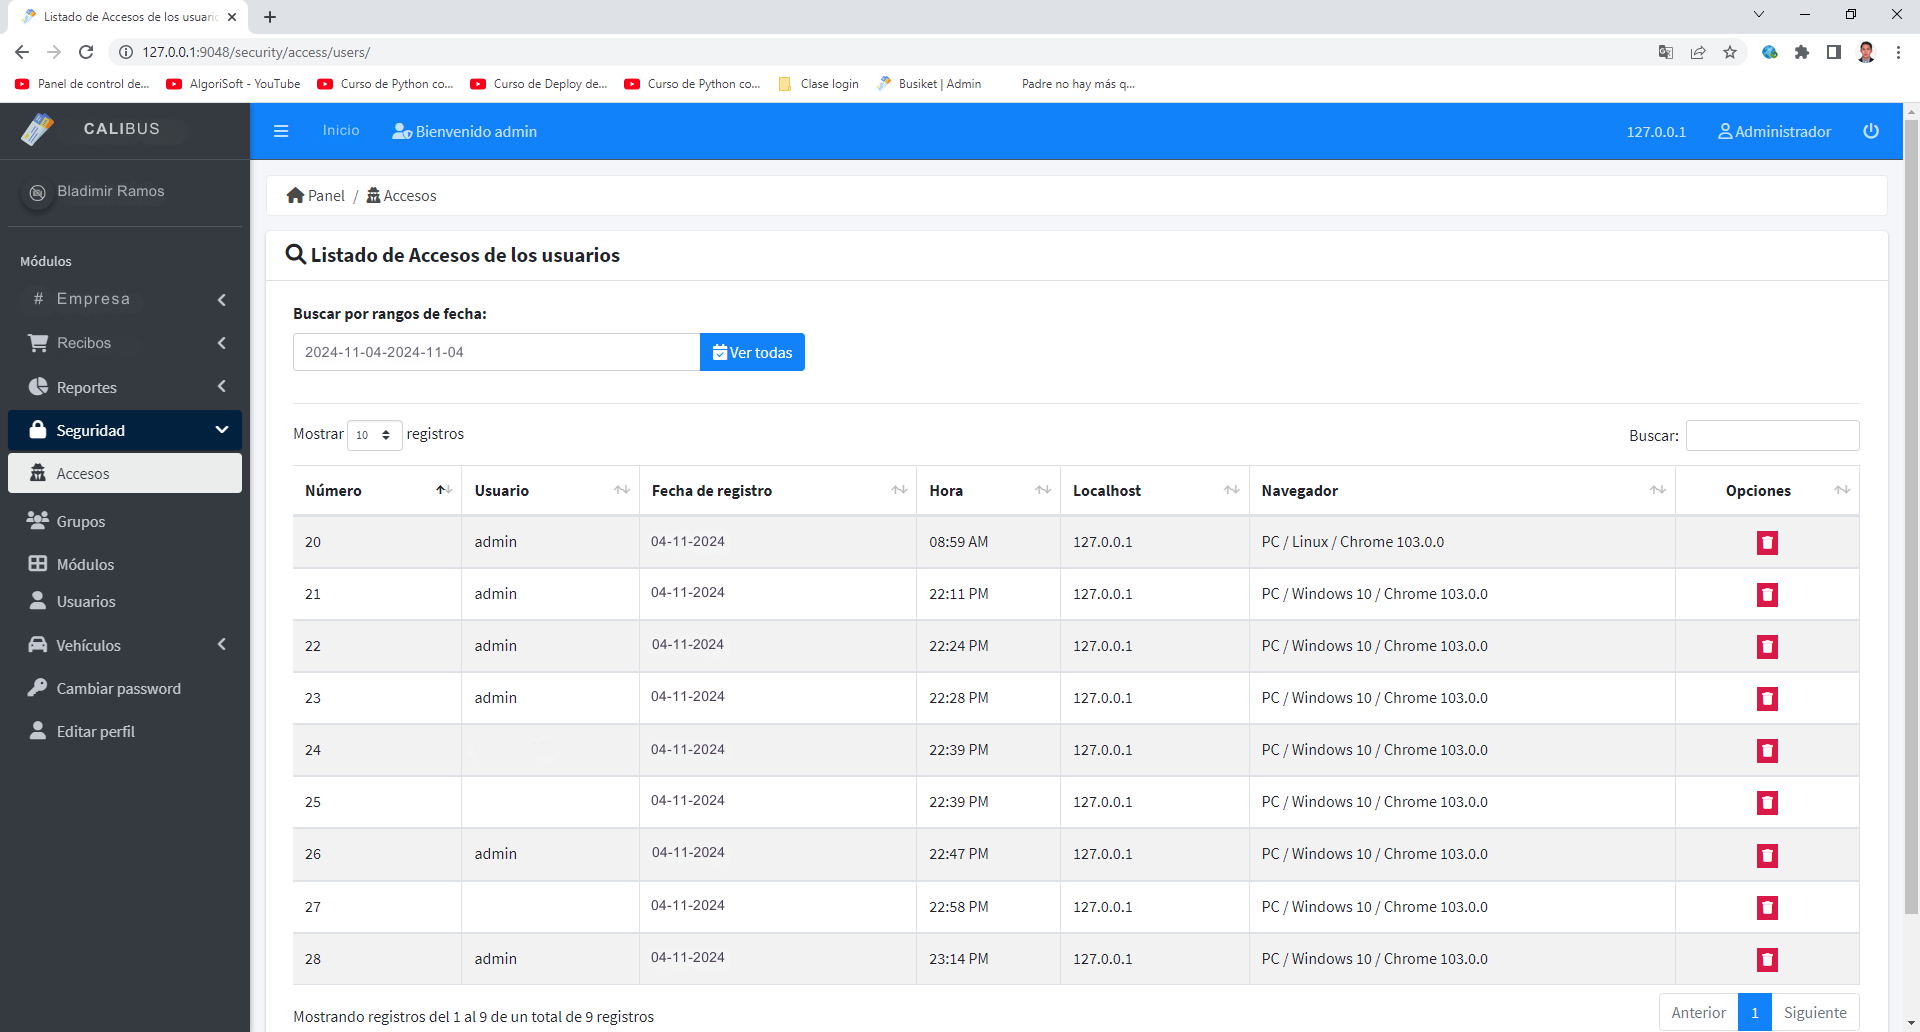
\includegraphics[width=0.83\textwidth]{imagenes/cap_3/Img_calibus/CALIBUS18.png} % Inserta una imagen
	
	\begin{flushleft}
		%\hspace{1.20cm} \textbf{Nota.} Organigrama obtenido en entrevista con el administrador. % Nota al pie para esta figura
	\end{flushleft}
	\vspace{-16pt}
	\label{fig:cali41} % Etiqueta para referencia cruzada
\end{figure}

\vspace{-0.6cm} % Agregar 1 cm de espacio entre el párrafo y la figura
